\documentclass{beamer}

\title{IT risk Management Strategy}
\subtitle{Key Steps}

%\usetheme{lucid}
\begin{document}
	\frame {
		\titlepage
	}
	\frame {
		\frametitle{The Steps}
IT risk management is the application of risk management methods to information technology to manage the risks inherent in that space. To do that means assessing the business risks associated with the use, ownership, operation and adoption of IT in an organization. Follow these steps to manage risk with confidence.
	}
	\frame{
		\frametitle{Identify the risks}

You can’t prepare for risk without first figuring out, to the best of your ability, where and when it might arise. Therefore, both manager and team must be alert to uncovering and recognizing any risks, then detailing them by explaining how they might \emph{impact} the project and outcomes. One method is using an IT risk assessment template.

\includegraphics[width=5cm]{./risk.jpg}



	}
	\frame{
	    \frametitle{Analyzing the risk}

Once you’ve identified risk, you then must analyze it and discern if it’s big, small or minimal in its \emph{impact}. Also, what would be the \emph{impact} for each of the risks. Study the risk and how it might influence the project in various ways. You’ll add these findings to your risk assessment.

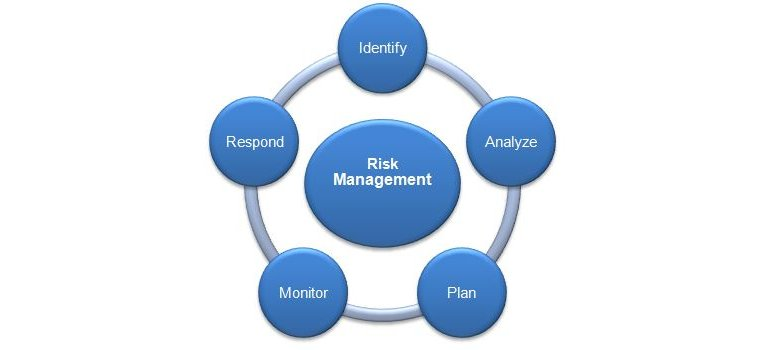
\includegraphics[width=5cm]{./Analysis.jpg}

	}


	\frame{
	    \frametitle{Evaluating the risk}

Once you evaluate the \emph{impact} of risks and prioritize them, you can begin to develop strategies to control them. This is done by understanding what the risk can do to the project, which is determining the \emph{likelihood} of it occurring and the magnitude of its \emph{impact}. Then you can say that the risk must be addressed or can be ignored without faulting the overall project. Again, these rankings would be added to your risk assessment.

	}


	\frame{
	    \frametitle{Respond the risk}

After all this, if the risk becomes an actual issue, then you’re no longer in the theoretical realm. It’s time for action. This is what’s called risk response planning in which you take your high-priority risks and decide how to treat them or modify them, so they place as lower priority. Risk mitigation strategies apply here, as well as preventive and contingency plans. Add these approaches to your risk assessment

	}


	\frame{
	    \frametitle{Monitor and Review the Risk}

Once you act, you must track and review the progress on mitigating the risk. Use your risk assessment to track and monitor how your team is dealing with the risk to make sure that nothing is left out or forgotten.


	}



\end{document}

    
